\documentclass{article}
\usepackage{tikz}

\begin{document}

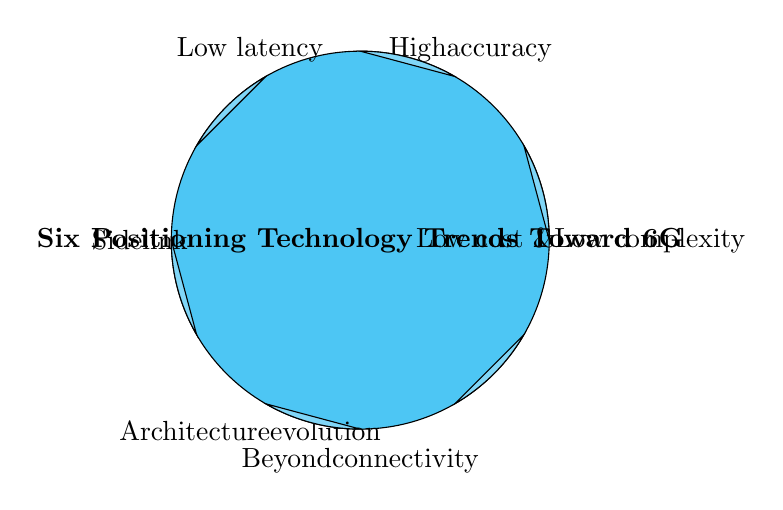
\begin{tikzpicture}[scale=0.8]
    \def\radius{3}
    \def\anglesep{60}
    
    % Draw the main circle
    \draw[fill=cyan!70] (0,0) circle (\radius);
    
    % Define the labels for each segment
    \node at (-90:\radius+0.5) {Beyond\\connectivity};
    \node at (0:\radius+0.5) {Low cost \&\\Low complexity};
    \node at (60:\radius+0.5) {High\\accuracy};
    \node at (120:\radius+0.5) {Low latency};
    \node at (180:\radius+0.5) {Sidelink};
    \node at (240:\radius+0.5) {Architecture\\evolution};
    
    % Draw the segments
    \foreach \i in {0,60,...,300} {
        \draw[fill=cyan!50] (\i:\radius) -- (\i+\anglesep/2:\radius) arc (\i+\anglesep/2:\i:\radius) -- cycle;
    }
    
    % Add the title
    \node at (0,0) {\textbf{Six Positioning Technology Trends Toward 6G}};
\end{tikzpicture}

\end{document}